\documentclass[11pt]{article}
% common.tex — minimal noise setup
% ----------------------------

% Silence package messages before anything else
\RequirePackage{silence}

% Completely hide "info" messages from LaTeX packages
\WarningFilter*{latex}{}
\WarningFilter*{hyperref}{}
\WarningFilter*{pgf}{}
\WarningFilter*{tikz}{}

% Optionally: hide some hyperref PDF string warnings that are common but harmless
\WarningFilter{hyperref}{Token not allowed in a PDF string}

% ----------------------------
% Now load the usual packages
\usepackage[utf8]{inputenc}
\usepackage[T1]{fontenc}
\usepackage{amsmath, amssymb, amsthm, amsfonts}
\usepackage{geometry}
\usepackage{hyperref}
\usepackage{graphicx}
\usepackage{physics}
\usepackage{booktabs}
\usepackage{listings}
\usepackage{bookmark}
\usepackage{amscd}
\usepackage{tikz-cd}
\usepackage{mathtools}
\usepackage{xspace}
\usepackage[backend=biber, style=numeric]{biblatex}
\usepackage{glossaries}
\usepackage{tcolorbox}

% ----------------------------
% Theorems, macros
\newtheorem{lemma}{Lemma}
\newcommand{\IaMe}{\(IaM^e\)\xspace}
\newcommand{\pdflink}[1]{}

% ----------------------------
% Page layout
\geometry{letterpaper, margin=1in}
\setlength{\parindent}{0pt}
\setlength{\parskip}{1em}

% Hyperref settings
\hypersetup{
    colorlinks=true,
    linkcolor=black,
    citecolor=black,
    filecolor=magenta,
    urlcolor=blue
}

% TOC formatting
\usepackage{tocloft}
\setlength{\cftbeforechapskip}{1.0em}
\setlength{\cftbeforesecskip}{0pt}
\setlength{\cftbeforesubsecskip}{0pt}
\renewcommand{\cftchapleader}{\cftdotfill{\cftdotsep}}

% Glossary
\defglsentryfmt{\ifglsused{\glslabel}{\glsgenentryfmt}{\textit{\glsgenentryfmt}}}

% Author
\author{$IaM^e$}


\input{../glossary.tex}
\addbibresource{../references.bib}

\title{\textbf{From Bitstring Simulations to Analytical Fields:\\
A Relational Cosmology Engine with Strict Information Conservation}}
\author{\textbf{Juha Meskanen} \\ \textit{The Abstract Universe Project}}
\date{June 2026}

\begin{document}

\maketitle

\begin{abstract}
This paper presents the Interactive Analytical Cosmology Engine, a macroscopic field-theoretic realization of the \iame{} framework. Moving from stochastic bitstring mutations to continuous lognormal density fields, the model enforces strict conservation of total information. The spacetime fabric density is defined as the residual after bound matter structures form. The observed cosmic scale factor emerges purely as a relational ratio between bound matter and free fabric, as perceived by internal observers. This framework reproduces qualitative features of cosmic expansion, including early rapid growth and late-time acceleration, in a simple, deterministic, and interactive manner.
\end{abstract}

\tableofcontents
\newpage

\section{Introduction}

The original Time-Reversed Entropic Cosmology simulation relied on a large bitstring evolved through random mutations, with hierarchical structures extracted via recursive pattern-matching filters. While conceptually powerful, this microscopic approach suffered from computational cost, discrete artifacts, and difficulty in exploring parameter space.

We therefore developed an analytical field model that captures the essential emergent statistics (lognormal abundance curves) while preserving the core ontological principles — in particular, the conservation of total information and the relational nature of measurement. This engine allows real-time interactive exploration of how different matter spectra affect the perceived cosmic expansion.

\section{Theoretical Framework}

\subsection{Information Conservation}

The universe is modeled as a closed informational system with a fixed total information capacity $I_{\text{total}}$. At any moment, this budget is partitioned between:

- Free spacetime fabric (vacuum / gravitons),
- Bound structures (hadrons, atoms, compounds).

The fabric density is not independent but defined as the residual:
\begin{equation}
\rho_{\text{fabric}}(t) = \max\left( I_{\text{total}} - \rho_{\text{matter}}(t),\ \epsilon \right)
\end{equation}

where $\rho_{\text{matter}}(t) = L_1(t) + L_2(t) + L_3(t)$, and each $L_k(t)$ is a lognormal density field representing one hierarchical level.

\subsection{Relational Scale Factor}

Internal observers can only measure distances using the emergent structures available to them. The perceived scale factor $R(t)$ is therefore defined relationally as:
\begin{equation}
R(t) = \frac{\rho_{\text{matter}}(t)}{\rho_{\text{fabric}}(t)}
\end{equation}

This formulation captures the Observer Matter Release Principle: when higher-order structures form, they consume free fabric, constraining the perceived space. When these structures later decay, they release information back into the fabric, causing the relational ratio (and thus the perceived size of space) to increase.

\subsection{Mechanism for $\Lambda$CDM-like Expansion}

This simple conservation law naturally generates rich dynamical behavior:

\textbf{1. Early Phase}: Rapid formation of matter pulls information from the fabric, initially constraining expansion.

\textbf{2.Intermediate Phase}: As matter reaches peak abundance, the scale factor grows more slowly.

\textbf{3. Late Phase}: Decay of bound structures returns information to the fabric. As $\rho_{\text{matter}} \to 0$, the denominator shrinks, driving the ratio $R(t)$ upward — producing late-time acceleration without any explicit cosmological constant.


\section{Model Implementation}

Each hierarchical level is represented by a normalized lognormal density field:
\begin{equation}
L_k(t) = A_k \cdot f_{\text{lognormal}}(t;\ \mu_k,\ \sigma_k)
\end{equation}

where the function is scaled so that the amplitude parameter $A_k$ directly corresponds to the true peak height, making parameter adjustment intuitive.

The matter fields are coupled through a cascading epoch system:
\begin{align*}
\mu_{\text{Hadron}} &= \mu_m \\
\mu_{\text{Atom}}   &= \mu_m + 0.8 \\
\mu_{\text{Compound}} &= \mu_m + 1.5
\end{align*}

with corresponding narrowing of widths to model progressive cooling and structure formation.

\section{User Manual: Dashboard Controls}

The interactive dashboard provides intuitive sliders divided into two groups.

\begin{figure}[h]
\centering
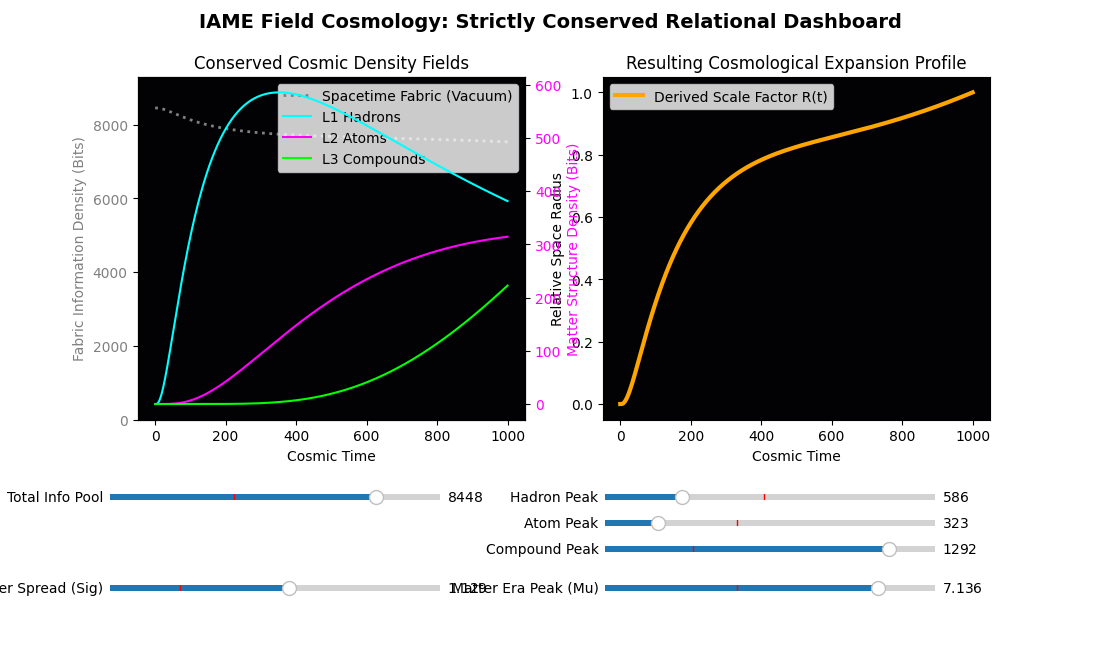
\includegraphics[width=1.0\textwidth]{figures/iace.png}
\caption{Lognormals for emergency of particles on the left. The resulting spacetime expansion on the right.}
\label{fig:iace}
\end{figure}


\subsection{Global Information Pool}

\textbf{Total Info Pool}: Controls the fixed total information budget $I_{\text{total}}$ of the universe.

\subsection{Matter Spectrum Controls}

\textbf{Hadron / Atom / Compound Peak}: True peak amplitudes of each hierarchical level.

\textbf{Matter Era Peak ($\mu_m$)}: Shifts the baseline timing for the entire matter cascade.

\textbf{Matter Spread ($\sigma_m$)}: Controls the overall width of the matter distributions (individual tiers are automatically scaled).

\section{Explorable Cosmological Regimes}

By adjusting the sliders, the engine can reproduce several qualitatively distinct expansion histories:

\begin{itemize}
\item \textbf{Standard $\Lambda$CDM-like evolutiond}: Balanced matter amplitudes with appropriate timing produce early expansion, a coasting phase, and late-time acceleration.
\item \textbf{Delayed Inflationary Bounce}: High total pool with delayed matter formation creates a long quiescent phase followed by rapid expansion.
\item \textbf{Big Crunch / Recollapse}: Strong late-time matter persistence or specific timing can produce a turnaround in the scale factor.
\end{itemize}

\section{Discussion}

This analytical engine demonstrates that many qualitative features of cosmic evolution can emerge from strict information conservation and relational measurement alone. It serves both as an exploratory tool for the \iame{} framework and as an intuitive demonstration of how expansion can be understood as a geometric consequence of internal observer dynamics rather than an absolute stretching of external space.

Future work will focus on quantitative fitting to observational data and tighter integration with the original bitstring simulation.

\section*{Supplementary Material}
The complete interactive Python implementation is available as \texttt{simulations/iace.py}.

\printbibliography

\end{document}

